% applications/bimalignment.tex

\chapter{BIM Alignment Modelling}

\label{chap:applications-bimalignment}

This chapter positions BIMalignment as an interoperability and workflow
application of AIM, not as a competing canonical architecture.

% ============================================================
\section{Application Context}
% ============================================================

BIM and exchange standards (for example IFC, LandXML, GIS-linked
containers) are essential project interoperability mechanisms. In AIM,
they are treated as representation and exchange layers downstream of
canonical engineering semantics.

The first figure answers the boundary question for this chapter: which
semantic layer owns engineering meaning, and which layer only represents
that meaning for exchange?

\begin{figure}[ht]
\centering
% figures/applications/support_canonical_vs_representation.tex
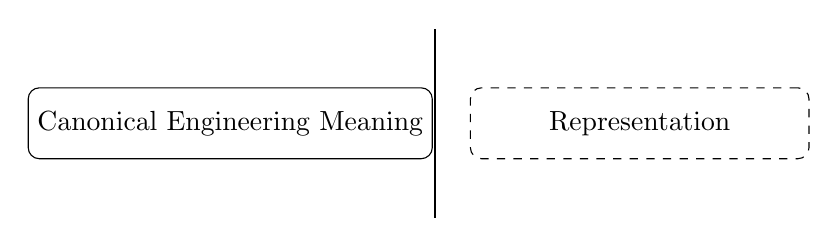
\begin{tikzpicture}[
  box/.style={draw, rounded corners, minimum width=4.3cm, minimum height=0.9cm, align=center},
  sec/.style={draw, rounded corners, dashed, minimum width=4.3cm, minimum height=0.9cm, align=center}
]
  \node[box] (canon) at (-2.6,0) {Canonical Engineering Meaning};
  \node[sec] (repr) at (2.6,0) {Representation};
  \draw[thick] (0,-1.2) -- (0,1.2);
\end{tikzpicture}

\caption{Supporting comparison: canonical engineering meaning and representation are distinct layers.}
\label{fig:support-canonical-vs-representation}
\end{figure}

The engineering consequence is that BIM workflows must consume canonical
AIM state and operators instead of redefining them in exchange schemas.

% ============================================================
\section{AIM-to-BIM Integration Role}
% ============================================================

BIMalignment in this thesis denotes alignment-centred integration where
AIM provides canonical semantics and runtime/realization evaluation,
while BIM-oriented structures provide object-oriented representation,
workflow integration, and lifecycle exchange.

\begin{principle}[BIM integration principle]
BIM integration consumes canonical AIM concepts and preserves their
ownership outside application chapters.
\end{principle}

% ============================================================
\section{Pipeline Interpretation}
% ============================================================

A typical interpretation pipeline is
\[
\text{exchange/import}
\rightarrow
\substack{\text{AIM normalization}\\\text{and evaluation}}
\rightarrow
\text{application consequence}
\rightarrow
\text{representation/export}.
\]

This keeps engineering objects and representations conceptually
separate.

The next figure addresses the interoperability question: how can native
and imported alignments be interpreted consistently under one canonical
state semantics?

\begin{figure}[ht]
\centering
% figures/applications/support_native_vs_imported.tex
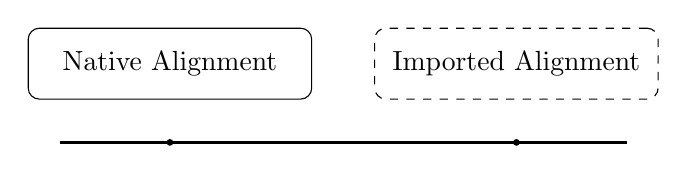
\begin{tikzpicture}[
  box/.style={draw, rounded corners, minimum width=3.6cm, minimum height=0.9cm, align=center},
  imp/.style={draw, rounded corners, dashed, minimum width=3.6cm, minimum height=0.9cm, align=center}
]
  \node[box] (native) at (-2.2,0) {Native Alignment};
  \node[imp] (imported) at (2.2,0) {Imported Alignment};
  \draw[thick] (-3.6,-1.0) -- (3.6,-1.0);
  \filldraw (-2.2,-1.0) circle (1.0pt);
  \filldraw (2.2,-1.0) circle (1.0pt);
\end{tikzpicture}

\caption{Supporting comparison: native and imported alignments require shared canonical interpretation.}
\label{fig:support-native-vs-imported}
\end{figure}

Its consequence is operational: import quality is assessed by canonical
semantic compatibility, not by format-level similarity alone.

% ============================================================
\section{Boundary Clarification}
% ============================================================

BIMalignment is not presented as a parallel state model. It is an
application-oriented integration strategy that depends on canonical
alignment semantics, pose2/pose3 interpretation, metric realization,
physical realization, and runtime services.

% ============================================================
\section{Connection to AIM}
% ============================================================

\begin{summary}
BIMalignment in this thesis is a downstream interoperability application
of AIM.

It demonstrates how canonical alignment-centred engineering semantics
can be connected to BIM/GIS exchange ecosystems without transferring
conceptual ownership away from the approved kernel architecture.
\end{summary}
